\chapter{Modelos}
\label{capitulo 2}

\section{Modelo Hidrológico}

\subsection{Modelo LEM}
Para obtener las series de caudales en régimen natural en la cuenca del río Chambo se ha empleado el 
modelo hidrológico  de equilibrio logístico, en adelante LEM, desarrollado por IHCantabria. 

Este modelo representa el proceso hidrológico a partir de las siguientes hipótesis empíricas:

\begin{enumerate}
    \item Las cuencas hidrográficas son sistemas complejos que persiguen continuamente un equilibrio dinámico, 
    dado por una combinación de factores climáticos ( precipitación y evapotranspiración potencial) 
    y algunas características del terreno (topografía, vegetación, suelo, geología, etc.). 

    La evolución de la escorrentía ($R$) hacia el equilibrio sigue la ley clásica de crecimiento descrito por la 
    ecuación logística:

    \begin{equation}
        \frac{d R(t)}{dt}=K\cdot R(t)\cdot\big(1-\frac{R(t)}{R_{eq}}\big)
    \label{eq.log}
    \end{equation}

    \item  $Req$ es la escorrentía de equilibrio  y se puede expresar como un coeficiente de escorrentía de 
    equilibrio ($Ceq$) multiplicado por la precipitación instantánea: $Req = P \cdot Ceq$. 
    
    \item $K$ es la tasa de crecimiento y es una función lineal de la precipitación: $K=P/S_0$ , donde $S_0$ 
    es una constante con unidades de longitud ($mm$) que representa un espesor característico del suelo.
    \item La ecuación logística no considera el  tiempo de viaje desde las 
    zonas de producción de escorrentía hasta el punto final de medida del caudal, en la salida de la cuenca. 
    Cuando el intervalo de tiempo de análisis es del mismo orden de magnitud que el tiempo 
    de respuesta de una cuenca, se debe agregar un método de propagación.


\end{enumerate}

La versión estándar del LEM adopta un modelo lineal para el submodelo de enrutamiento y toma la forma del siguiente sistema de 
ecuaciones:


\begin{equation}
    \frac{d R(t)}{dt}=\frac{P(t)}{S_0}\cdot R(t)\cdot\big(1-\frac{R(t)}{R_{eq}}\big)
\end{equation}

\begin{equation}
    \frac{d \hat{P}}{dt}=\frac{P(t)-\hat{P}}{\lambda}
\end{equation}


\begin{equation}
    \frac{d \hat{E}}{dt}=\frac{E(t)-\hat{E}}{\lambda}
\end{equation}


\begin{equation}
    R_{eq}(t)=P(t)\cdot C_{eq}(\psi);\ \ C_{eq}(\psi)=e^{-a\cdot \psi}, \psi=\frac{\hat{E}}{\hat{P}}
\end{equation}


\begin{equation}
    \frac{d Q(t)}{dt}=\frac{1}{\tau}K\cdot \big[R(t)-Q(t)\big]
\end{equation}


Donde $R$ y $Q$ son la escorrentía total y la descarga medida en la salida de la cuenca, respectivamente. 
$P$ y $E$ son la precipitación y la evapotranspiración potencial en cada paso de tiempo, mientras que $\hat{P}$ y $\hat{E}$ 
son valores promediados de $P$ y $E$ durante un periodo de tiempo característico, respectivamente. 
Los parámetros del modelo son:

\begin{itemize}
    \item $\lambda$ (días), el tiempo característico de respuesta  de la cuenca ($1/(25.465*log(s0)-19.494)$).
    \item $S_0$ (mm), que representa un espesor medio de suelo o una capacidad de almacenamiento característica de la cuenca.
    \item $a$, un parámetro adimensional que modifica la forma de la función de equilibrio (típicamente en el rango 0.5-1.5)
    \item $\tau$ (horas), el parámetro de enrutamiento, que puede considerarse un tiempo 
    de respuesta rápido de la cuenca.
\end{itemize}

Este sistema de ecuaciones diferenciales ordinarias puede resolverse numéricamente con un esquema explícito 
incondicionalmente estable, ya que  que todas las ecuaciones, y en especial la logística, tienen solución analítica.

\subsection{Modelo MELCA}

MELCA es un modelo hidrológico semi-distribuido basado en LEM. 
Este modelo considera varias subcuencas, cada una de ellas con sus parámetros y forzamientos climáticos diferenciados
y permite incluir una serie de particularidades asociadas a las cuencas tropicales andinas como la inclusión de páramos 
y bofedales con sus topologías y estado de conservación. El modelo convierte la superficie de cada uno de estos 
ecosistemas andinos en una capacidad equivalente de almacenamiento del suelo. 
También  incluye factores de corrección para  la evotranspiración en zonas de alta montaña, el efecto de glaciares 
y la aportación de agua atmosférica proveniente de niebla (flujo que es significativo en zonas cuencas andinas tropicales). 

\subsection{Parámetros físicos}
% Tanto el modelo MELCA  usa 5 parámetros de entrada, el área de la cuenca, 
% el almacenamiento característico $s_0$, el parámetro de enrutamiento $\tau$, 
% el factor corrector de las precipitaciones $fcp$ y el factor corrector de la evotranspiración $fce$. 

\subsubsection{Capacidad de almacenamiento}
La capacidad de almacenamiento del terreno se ha estimado mediante el método del Número de 
Curva del \textit{Soil Conservation Service} (SCS).

Si consideramos que para una cantidad de precipitación $P$, una cantidad $P_e$ se escurre directamente y una cantidad
$I_a$ se infiltra inicialmente. Por otro lado, una cantidad de agua $F_a$ es retenida y es  
menor a la capacidad máxima de almacenamiento de la cuenca $S_{max}$.

El método SCS supone que entre todas las cantidades descriptas, se satisface la siguiente relación:
\begin{equation}
    \frac{F_a}{S_{max}}=\frac{P_e}{P-I_a}
\end{equation}

Si además aplicamos el principio de continuidad para la precipitación, $P = P_e+I_a+F_a$ y la relación experimental
entre $S_{max}$ y $I_a$, $I_a=0,2\cdot S_max$, obtenemos una relación entre $P_e$ y $S_{max}$:

\begin{equation}
    P_e=\frac{(P-0,2\cdot S_{max})^2}{P-0,8\cdot S_{max}}
\end{equation}


El número de curva (CN) se relaciona con la capacidad de almacenamiento máxima de la cuenca de la siguiente manera:

\begin{equation}
    S_{max}=25,4\cdot\bigg(\frac{1000}{CN}-10\bigg)
\end{equation}

Los números de curva se encuentran tabulados en función del tipo y uso del suelo (referencia).

Una vez conocidas las capacidades máximas de almacenamiento del suelo por subcuencas, podemos calcular el 
almacenamiento característico $S_0$, tal y como lo requiere el modelo LEM, antes descrito. 
De acuerdo a la experiencia de aplicación del modelo en otras cuencas, podemos asumir con  con buen grado de 
ajuste la siguiente relación:

\begin{equation}
    S_{max}=9\cdot S0
\end{equation}

\subsubsection{Coeficiente de enrutamiento}

El parámetro de enrutamiento $\tau$ representa el retardo entre la generación 
de la escorrentía en el territorio y su llegada al punto de medida en el final de cada tramo. Este parámetro 
tiene muy poca influencia en el cálculo de los recursos hídricos, ya que no altera el balance de masa, sino que 
retrasa ligeramente la llegada del caudal (unas horas, mientras que el paso de tiempo de cálculo es un día). 

\subsubsection{Factores correctores de las precipitaciones}
Como se ha mencionado en el capítulo \ref{capitulo 1}, los datos de precipitación correspondientes a las zonas más 
altas de la cuenca son escasos. Es por esto que es necesario aplicar un factor de corrección, $fcp$, a las series de precipitación
que tiene en cuenta la influencia de la altitud de cada subcuenca, en general las subcuencas que se encuentran a mayor
altitud tendrán un factor de corrección mayor. 

\subsubsection{Cálculo de la evapotranspiración corregida}

La evapotranspiración potencial (ETP) se ha calculado con base en la fórmula de la FAO 56 PM (referencia), 
que toma los datos de temperatura máxima y mínima de rásteres en cada subcuenca:

\begin{equation}
    ETP_0\bigg(\frac{mm}{d}\bigg)=\frac{12,64}{365,25}\cdot \bigg(T_{med}+17,8\bigg)\cdot\bigg(T_{max}-T_{min}\bigg)^{0,5}
\end{equation}

Para calcular las temperaturas máximas y mínimas diarias, Tmax y Tmin, se han usado las interpolaciones de los datos 
instrumentales y la base de datos de ERA5 \ref{tempint}.


En las cuencas ecuatorianas andinas, la fórmula anterior tiende a sobreestimar la ETP en hasta un 30 $\%$ (Córdova,2015),
ya que no considera el efecto del aumento de radiación solar ni las condiciones locales de humedad relativa y por otro lado 
la presencia de viento en esas zonas también distorsiona el valor de ETP. Por lo tanto, se ha aplicado un factor corrector al 
resultado de la fórmula de la FAO que depende de la altitud y orientación de cada cuenca:

\begin{equation}
    ETP\bigg(\frac{mm}{d}\bigg)=f_{ce}\cdot ETP_0\bigg(\frac{mm}{d}\bigg)
\end{equation}

\subsubsection{Calibración del modelo}
Para calibrar el modelo se han utilizado datos de caudales recogidos por diferentes estaciones de aforo proporcionados por
MAATE (REF) y los valores de caudal promedio aportados por el documento de Aportes a la planificación para la gestión integral 
de los recursos hídricos de Rodríguez, J. (2015). 
El modelo es entonces calibrado ajustando los factores de corrección $fcp$ y $fce$ de manera tal que los caudales mensuales medios 
simulados se acerquen lo máximo posible a los valores medidos en las estaciones de aforo.


\begin{figure}[h!]
    \begin{center}
      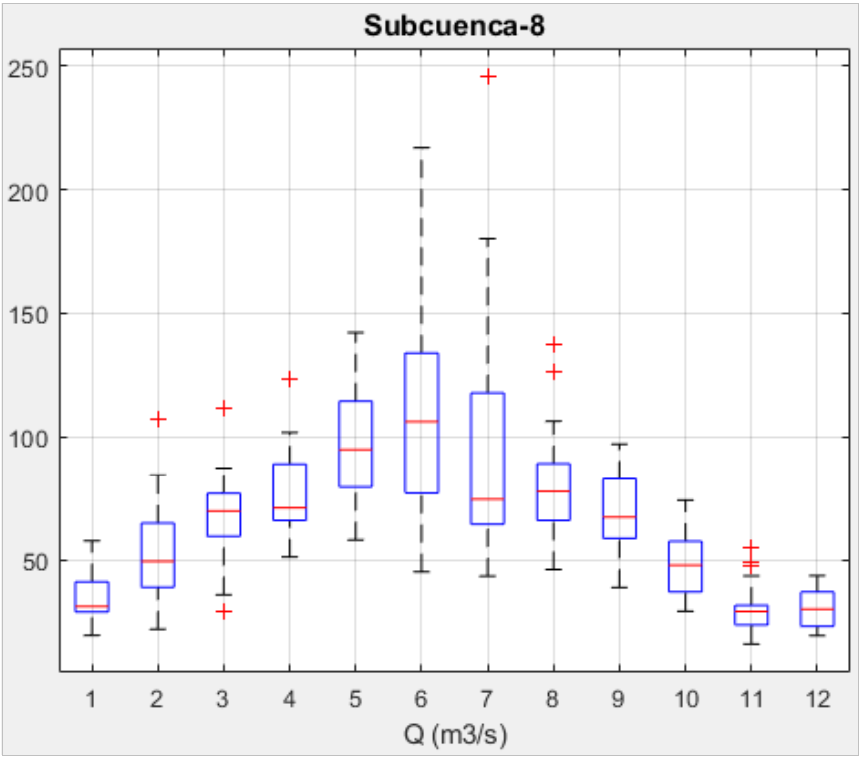
\includegraphics[height=3.in]{Figures/caudal_sim.PNG}
      \caption{ Valores simulados de caudales mensuales para la subcuenca 8.}
      \label{2}
    \end{center}
  \end{figure}



 \begin{figure}[h!]
    \begin{center}
      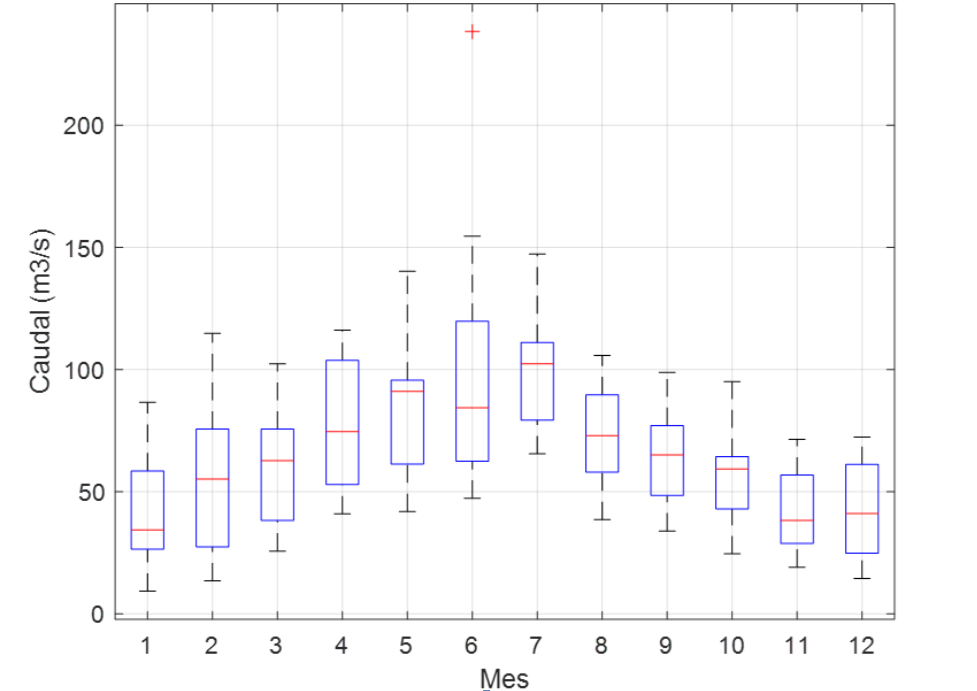
\includegraphics[height=3.in]{Figures/caudal_obs.PNG}
      \caption{ Valores observados de caudales mensuales para la subcuenca 8.}
      \label{3}
    \end{center}
  \end{figure}



  En la figura \ref{2} se muestran a modo de ejemplo, los valores observados (panel inferior) y simulados  (panel superior) para la subcuenca 8.
  La línea roja representa el valor medio, la caja azul representa los valores situados entre los percentiles
  25$\%$ y 75$\%$, y las barras negras los extremos (los puntos en rojo son tratados como datos atípicos). 
   Se puede observar que a calibración ha ayudado a igualar considerablemente los caudales modelados con los caudales aforados.


\subsubsection{Resultados obtenidos con MELCA}



  

\begin{figure}[h!]
    \begin{center}
      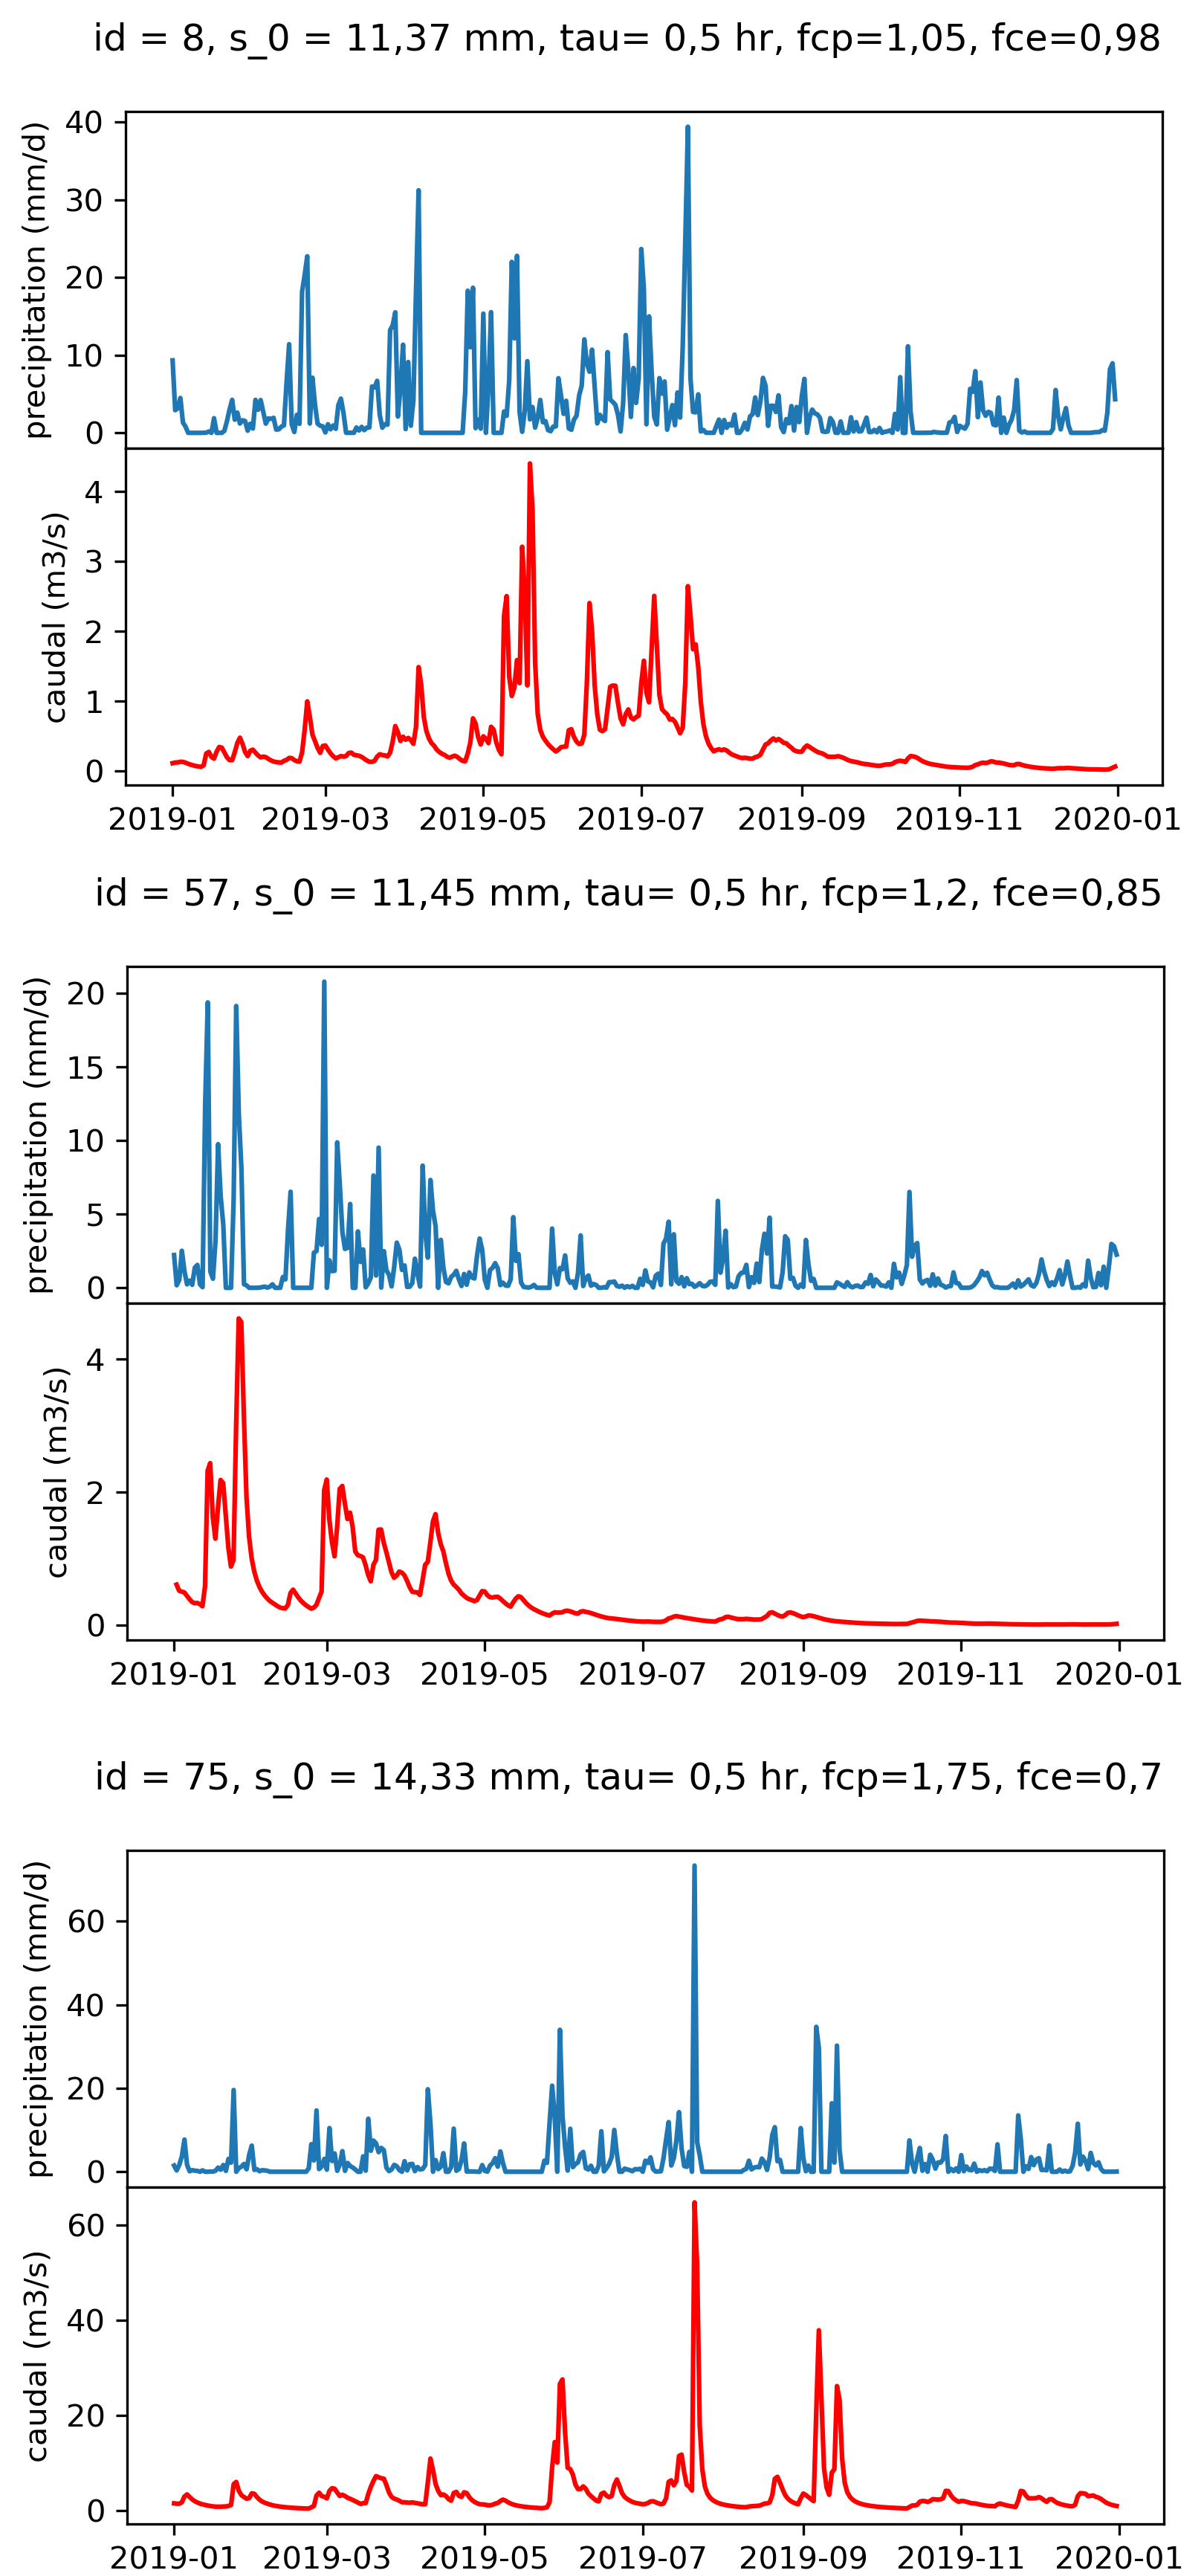
\includegraphics[height=6.5in]{Figures/outputs_MELCA.png}
      \caption{ Simulaciones de caudales naturales para tres subcuencas durante el añ0 2019, 
      en las graficas superiores se muestran las series de 
      precipitación de entrada y los parámetros del modelo.}
      \label{5}
    \end{center}
  \end{figure}

  \begin{figure}[h!]
    \begin{center}
      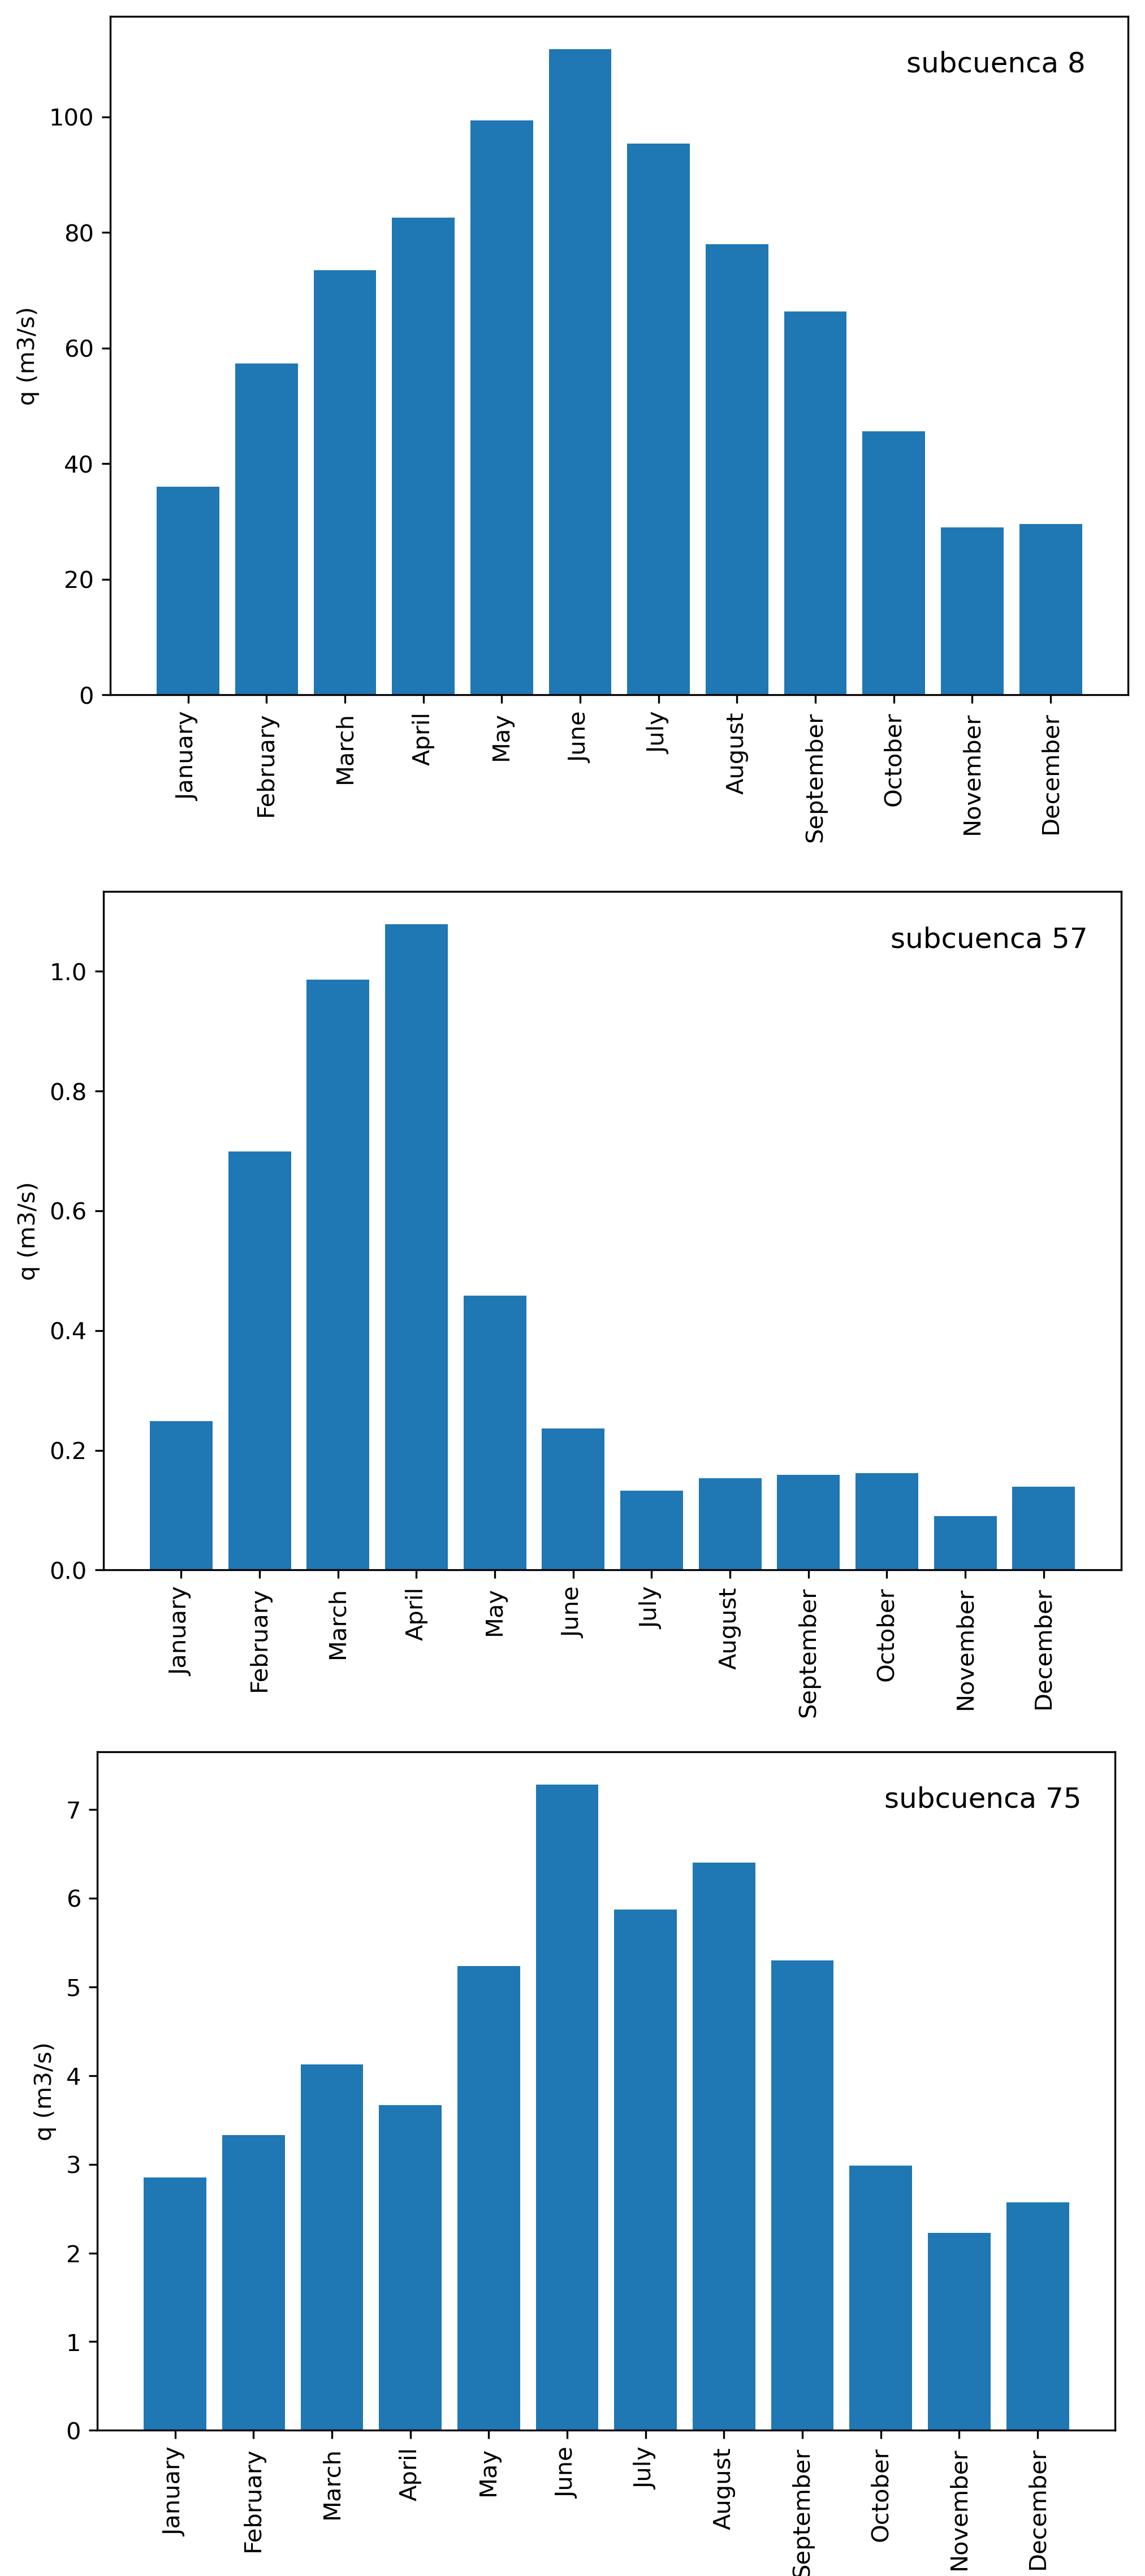
\includegraphics[height=6.5in]{Figures/outputs_MELCA_mensuales.png}
      \caption{ Valores medios mensuales de caudal natural para tres subcuencas durante los años 2000 y 2020.}
      \label{6}
    \end{center}
  \end{figure}

 En la figura \ref{5} se muestran graficas con los resultados  para 
las subcuencas con id 8, 57 y 75 (ver figura \ref{4}). 
En los paneles superiores se muestras las series de precipitación de entrada y los parámetros del modelo, 
capacidad de almacenamiento,
coeficiente de enrutamiento y los factores de corrección. 
La cuenca más alta es la 75 (?) y posee el mayor factor de corrección fcp,
la más baja es la 8 y tiene el factor de corrección menor.

Tal y como vimos en la sección \ref{regimenes_prec}, la subcuenca 8 presenta un regimen de precipitaciones 
mixto, de las tres cuencas es la que se encuentra más aguas abajo por lo que el caudal medio, ---, es 
considerablemente superior que en las otras dos. Su area es de --
la superficie agregada de la cuenca es de --- 
(sumando la superficie de las cuencas aguas arriba que vierten ella) lo que se produce en una productividad de ---.
La cuenca 57 se encuentra en la region oeste, presente un regimen bimodal, caudal medio de ---, superficie --- y 
productividad media de ---, mientras que la cuenca 75 presenta un régimen monomodal y sus valores son---, ---
y respectivamente.



En la figura ... se muestran los caudales medios mensuales
para la salida de la cuenca (subcuenca 73) . El caudal medio es de --- $m^3/s$ 
este asciende a un valor máximo de ...entre los meses de ... y de ...., y presenta un mínimo de .... entre los meses de ....
y ..... La superficie agregada de la cuenca es de 3590 $km^2$, con una precipitación media de 1120 $mm$ que se traducen en una 
productividad de ----.

\textcolor{codegreen}{(agregar caudales de escorrentía para cada una)}
  

% \subsection{Parámetros físicos}
% \subsubsection{Capacidad máxima de almacenamiento del terreno}

% Las ecuaciones anteriores pueden aplicarse de manera agregada para toda una cuenca, considerada como un ente único, 
% o bien de manera semi-distribuida, considerando varias subcuencas, cada una de ellas con sus parámetros y forzamientos 
% climáticos diferenciados. Si se emplea el modelo en un marco semi-distribuido, es preciso incluir, cuando el paso temporal
%  de cálculo lo requiera, la traslación del flujo desde cada subcuenca al punto de salida. El MELCA es precisamente una 
%  versión semi-distribuida del LEM genérico,
%  con una serie de particularidades que se describen a continuación.

\section{Modelado de balance hidrológico}
\label{Modelo_balance}

Una vez obtenidos los caudales naturales y las demandas en la cuenca del río chambo se pueden calcular los caudales intervenidos
fluyentes por los tramos de ríos. Para un primer análisis se ha creado un software que calcula para cada una de las subcuencas
el resultado final de forma agregada teniendo en cuenta los flujos de entrada proveniente de las subcuencas aguas arriba, 
el flujo del caudal natural local, las demandas de agua en dicha subcuenca y  el caudal de retorno de las demandas que vierten a ese tramo.
Cabe destacar que para este primer análisis no se han establecido criterios de prioridades de las demandas por lo cual 
no nos centraremos en un problema de optimización, en cambio consideraremos que todas las demandas tienen las mismas 
prioridades.

\begin{equation}
    q_{total} = q_{entrada}+q_{natural}-q_{demandas}+q_{retornos}
    \label{caudal_tot}
\end{equation}

\begin{figure}[h!]
    \begin{center}
      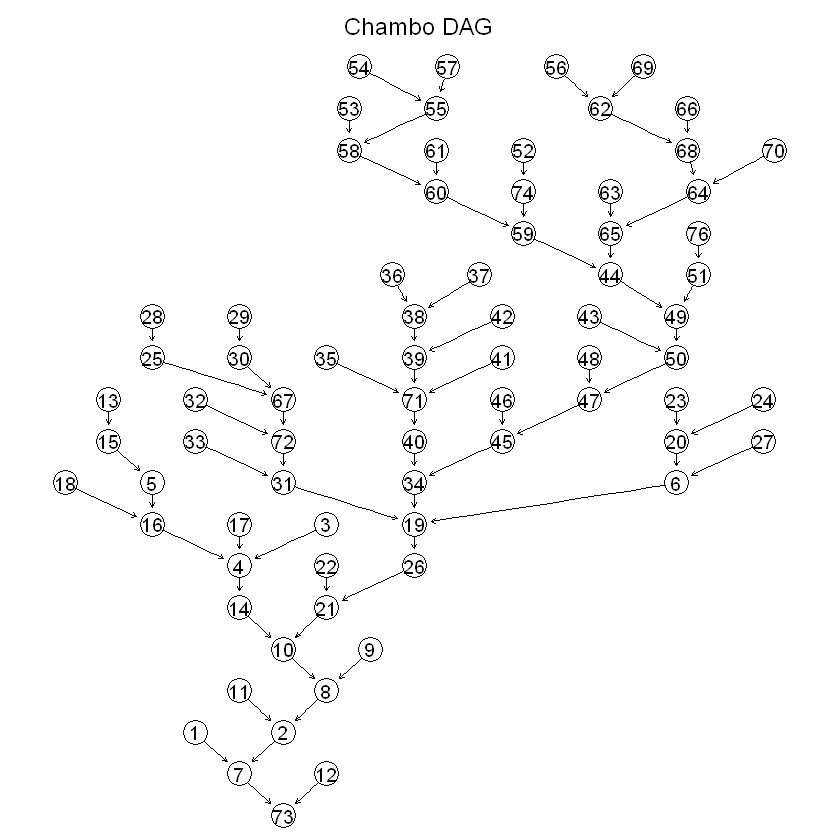
\includegraphics[height=5.in]{Figures/modelo_conceptual_cuenca.png}
      \caption{Modelo conceptual del entramado de los tramos de la cuenca del río Chambo.}
      \label{6}
    \end{center}
  \end{figure}

En la figura \ref{6} se muestra una representación conceptual de la cuenca, donde se puede seguir el recorrido de los 
flujos de aguay la estructura lógica que conecta las diferentes subcuencas y usos de agua. Y en la figura \ref{7} se muestra el 
diagrama de flujos del programa que calcula el balance hidrológico para cada subcuenca. Este programa realizado en python, 
realiza las siguientes acciones:

\begin{enumerate}
    \item ejecuta el modelo MELCA, cuyo resultado son las series con los caudales para todas las subcuencas de Chambo y selecciona
    la serie correspondiente al id de la subcuenca de estudio.
    \item utilizando la matriz de conectividades, cuyas filas  son las cuencas receptoras y cuyas columnas las cuencas 
    tributarias (ver figura ...) encuentra los ids de las cuencas tributarias.
    \item encuentra para cada uno de estos ids las demandas totales, seleccionando las filas que satisfacen la condiciones
    INIC=id (ver tabla demandas) y las agrega. 
    \item de manera similar calcula los retornos totales, pero esta vez aplicando la condición  FIN=id sobre la tabla demandas 
    ya que los caudales de retorno son los flujos vertidos aguas abajo por las demandas
    \item Encuentra las demandas ecosistémicas para cada uno de estos ids y las agrega.
    \item calcula el resultado final  como en la ecuación \ref{caudal_tot}.
\end{enumerate}


A modo de ejemplo, si queremos calcular el caudal resultante para la sub cuenca 68, entonces las cuencas tributarias son las 66 y 62
(ver figura \ref{6}), estas se obtienen al imponer la condición a la matriz de conectividades, $matcon[66,:]==1$. Una vez se obtienen
los ids de las cuencas tributarias, se procede a calcular el caudal final como se explica en los puntos 3-6.


\begin{figure}[h!]
    \begin{center}
      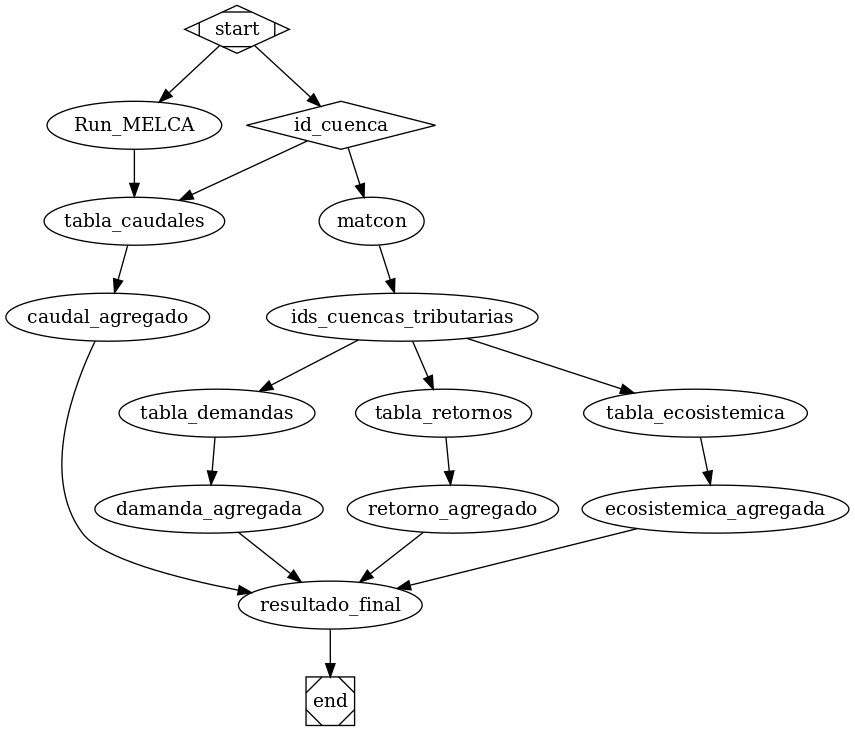
\includegraphics[height=5.in]{Figures/graphviz.png}
      \caption{Diagrama de flujos del programa que calcula el balance hidrológico de la cuenca.}
      \label{7}
    \end{center}
  \end{figure}

\section{Modzin}

% Formato de código desde un archivo.

% \vspace{0.7cm}
% \lstinputlisting[style=codigo,language=bash,caption=ejemplo1.sh]{codigo_fuente/ejemplo1.sh}
% \vspace{0.7cm}

% Otro formato de código, para utilizar como salida de ejecución.

% \vspace{0.7cm}
% \begin{lstlisting}[style=terminal,caption=Salida del ejemplo1.sh]
% $ ./ejemplo1.sh 
% 1
% 2
% 3
% 4
% 5
% 6
% 7
% 8
% 9
% 10
% \end{lstlisting}
% \vspace{0.7cm}